\documentclass[10pt,openany]{book}
% ------------------------------------------------------------
% Preamble for 「Pythonによる はじめての銀河シミュレーション」
% 157 x 221 mm layout based on the supplied textbook template.
% Compile with XeLaTeX.
% ------------------------------------------------------------
\usepackage[paperwidth=157mm,paperheight=221mm,margin=14mm,headheight=14pt,headsep=6mm]{geometry}
\usepackage{amsmath,amssymb,mathtools,bm}
\usepackage{graphicx,rotating,float,placeins,caption}
\captionsetup{font=small,labelfont=bf,labelsep=quad}
\graphicspath{{figures/}{./}}
\usepackage{fontspec}
\usepackage{xeCJK}
\IfFontExistsTF{Latin Modern Roman}{\setmainfont{Latin Modern Roman}}{\setmainfont{Liberation Serif}}
\IfFontExistsTF{Latin Modern Sans}{\setsansfont{Latin Modern Sans}}{\setsansfont{Liberation Sans}}
\IfFontExistsTF{DejaVu Sans Mono}{\setmonofont{DejaVu Sans Mono}[Scale=0.91]}{}
\setCJKmainfont{Noto Serif CJK JP}[ItalicFont={Noto Serif CJK JP}]
\setCJKsansfont{Noto Sans CJK JP}
\setCJKmonofont{Noto Sans Mono CJK JP}[Scale=0.90]
\xeCJKsetup{CJKmath=true}
\XeTeXlinebreaklocale "ja"
\XeTeXlinebreakskip = 0pt plus 0.1pt minus 0.01pt

\usepackage{xcolor,enumitem,array,booktabs,tabularx,xurl,etoolbox,needspace,fvextra}
\usepackage{fix-cm}

% TikZ settings are defined here rather than in a separate input file.
% This makes the project robust on Overleaf even when only the main preamble
% and chapter/figure files are copied into an existing project.
\usepackage{tikz}
\usetikzlibrary{arrows.meta,calc,positioning,patterns,decorations.pathreplacing,matrix}
\definecolor{figblue}{HTML}{0072B2}
\definecolor{figred}{HTML}{D55E00}
\definecolor{figgreen}{HTML}{009E73}
\definecolor{figgray}{HTML}{666666}
\tikzset{
  textbook diagram/.style={font=\sffamily\fontsize{9}{11}\selectfont,>=Latex,line width=0.6pt},
  vector/.style={-{Latex[length=2.1mm,width=1.4mm]},line width=0.85pt},
  guide/.style={draw=figgray,densely dashed,line width=0.5pt},
  state/.style={draw=black!50,fill=white,rounded corners=1pt,minimum width=48mm,minimum height=9mm,align=center},
  hint/.style={align=left,font=\sffamily\fontsize{8.5}{10.5}\selectfont},
  small label/.style={font=\sffamily\fontsize{8}{10}\selectfont}
}

\usepackage[most]{tcolorbox}
\usepackage{listings}
\usepackage{titlesec,fancyhdr}

\setlength{\parindent}{1em}
\setlength{\parskip}{0.15em}
\linespread{1.08}
\raggedbottom
\emergencystretch=1.5em
\widowpenalty=10000
\clubpenalty=10000

\definecolor{navy}{HTML}{0D1B3E}
\definecolor{amber}{HTML}{B5740F}
\definecolor{amberbg}{HTML}{FBF1E0}
\definecolor{cyan}{HTML}{1F6390}
\definecolor{cyanbg}{HTML}{E7F0F7}
\definecolor{navybg}{HTML}{EDF0F7}
\definecolor{rule}{HTML}{C9D2E3}
\definecolor{notegray}{HTML}{F3F5F6}
\definecolor{notegreen}{HTML}{287250}
\definecolor{warnred}{HTML}{9B4030}

% Article boxes: notebox/failbox. goalbox is a chapter-opening structural element.
\newtcolorbox{notebox}[1]{enhanced,breakable,colback=notegray,colframe=notegreen,
  boxrule=0.45pt,arc=1.5pt,left=2.8mm,right=2.8mm,top=2mm,bottom=2mm,
  fonttitle=\sffamily\bfseries,colbacktitle=notegreen!10,coltitle=notegreen,
  title={もう少し詳しく：#1},before skip=7pt,after skip=7pt}
\newtcolorbox{failbox}[1]{enhanced,breakable,colback=notegray,colframe=warnred,
  boxrule=0.45pt,arc=1.5pt,left=2.8mm,right=2.8mm,top=2mm,bottom=2mm,
  fonttitle=\sffamily\bfseries,colbacktitle=warnred!8,coltitle=warnred,
  title={よくある失敗：#1},before skip=7pt,after skip=7pt}
\newtcolorbox{goalbox}[1][本章の目標]{colback=cyanbg,colframe=cyan,coltitle=white,
  title={\sffamily #1},fonttitle=\bfseries,boxrule=0.7pt,arc=2pt,
  left=7pt,right=7pt,top=5pt,bottom=5pt,breakable}

\newcommand{\inputcode}[1]{\par\smallskip\noindent\begin{minipage}{\linewidth}\VerbatimInput[
  fontsize=\fontsize{7.5}{9.3}\selectfont,frame=lines,rulecolor=\color{navy!35},framesep=2.2mm,
  numbers=left,numbersep=4pt,breaklines=true,breakanywhere=true,tabsize=4]{generated/#1.py}\end{minipage}\par\smallskip}

\titleformat{\chapter}{\LARGE\bfseries\sffamily\color{navy}}{第\thechapter 章}{0.8em}{}
\titleformat{\section}{\large\bfseries\sffamily\color{navy}}{\thesection}{0.5em}{}
\titleformat{\subsection}{\normalsize\bfseries\sffamily\color{navy}}{\thesubsection}{0.5em}{}
\titlespacing*{\chapter}{0pt}{0pt}{12pt}
\titlespacing*{\section}{0pt}{1.1em}{0.4em}
\titlespacing*{\subsection}{0pt}{0.75em}{0.25em}
\pretocmd{\section}{\Needspace{6\baselineskip}}{}{}
\pretocmd{\subsection}{\Needspace{5\baselineskip}}{}{}
\setlist[itemize]{leftmargin=1.7em,itemsep=0.15em,topsep=0.25em}
\setlist[enumerate]{leftmargin=2em,itemsep=0.2em,topsep=0.3em}
\setcounter{tocdepth}{1}
\setcounter{secnumdepth}{2}

\pagestyle{fancy}
\fancyhf{}
\fancyhead[L]{\scriptsize\sffamily はじめての銀河シミュレーション}
\fancyhead[R]{\scriptsize\sffamily\nouppercase{\leftmark}}
\makeatletter
\renewcommand{\chaptermark}[1]{%
  \if@mainmatter
    \markboth{第\thechapter 章\enspace #1}{}%
  \else
    \markboth{#1}{}%
  \fi}
\makeatother
\fancyfoot[R]{\small\thepage}
\fancypagestyle{plain}{\fancyhf{}\fancyfoot[R]{\small\thepage}\renewcommand{\headrulewidth}{0pt}}

\newcommand{\rvec}{\boldsymbol r}
\newcommand{\vvec}{\boldsymbol v}
\newcommand{\avec}{\boldsymbol a}
\newcommand{\yvec}{\boldsymbol y}
\newcommand{\fvec}{\boldsymbol f}
\newcommand{\kvec}{\boldsymbol k}
\newcommand{\Rvec}{\boldsymbol R}
\newcommand{\Vvec}{\boldsymbol V}
\newcommand{\Dvec}{\boldsymbol D}
\newcommand{\Uvec}{\boldsymbol U}
\newcommand{\Pvec}{\boldsymbol P}
\newcommand{\Mtot}{M_{\rm tot}}
\newcommand{\mred}{m_{\rm red}}
\newcommand{\Tc}{T_{\rm c}}
\newcommand{\Msun}{M_\odot}
\newcommand{\unit}[1]{\,\mathrm{#1}}
\newcommand{\dd}{\mathrm{d}}
\newcommand{\vect}[1]{\boldsymbol{#1}}
\newcommand{\figpath}[1]{figures/#1.pdf}
\renewcommand{\contentsname}{目次}
\renewcommand{\figurename}{図}
\renewcommand{\tablename}{表}
\renewcommand{\bibname}{参考図書}
% Chapter zero must keep the prefix in figures, tables, and equations.
\renewcommand{\thefigure}{\thechapter.\arabic{figure}}
\renewcommand{\thetable}{\thechapter.\arabic{table}}
\renewcommand{\theequation}{\thechapter.\arabic{equation}}
% Same end-of-chapter headings and bibliography in every chapter.
\newcommand{\chapterexercises}{\section*{演習}\phantomsection\addcontentsline{toc}{section}{演習}}
\newcommand{\answerchapter}[2]{\section*{第#1章　#2}\phantomsection\addcontentsline{toc}{section}{第#1章　#2}}
% Shell commands are not executable Python; keep them visibly distinct.
\newcommand{\inputterminal}[1]{\par\smallskip\noindent
  {\footnotesize\sffamily 端末で実行}\par\nobreak
  \VerbatimInput[fontsize=\fontsize{8}{10}\selectfont,frame=single,rulecolor=\color{black!30},
  framesep=2mm,breaklines=true,breakanywhere=true,numbers=none]{#1}\smallskip}
\newcommand{\booktitle}{Pythonによる はじめての銀河シミュレーション}
\newcommand{\booksubtitle}{テスト粒子で学ぶ重力・軌道・銀河相互作用}
\newcommand{\bookversion}{見出し統一版 v2.5}
\newcommand{\distributionnote}{授業・ゼミで案内する配布先から入手してください。公開URLは刊行時に確定します。}


\renewcommand{\topfraction}{0.95}
\renewcommand{\bottomfraction}{0.85}
\renewcommand{\textfraction}{0.05}
\renewcommand{\floatpagefraction}{0.85}
\setcounter{topnumber}{3}
\setcounter{totalnumber}{5}
\setlength{\textfloatsep}{9pt plus 3pt minus 2pt}
\setlength{\intextsep}{9pt plus 3pt minus 2pt}

\usepackage[unicode,colorlinks=true,linkcolor=cyan,citecolor=cyan,urlcolor=cyan]{hyperref}

\begin{document}
\pagestyle{plain}
\renewcommand{\thefigure}{A\arabic{figure}}
\captionsetup{hypcap=false}
\noindent{\Large\sffamily\bfseries KDKの更新順序}\par\medskip
\noindent{\small 本文の対応箇所：1.5.2節}
\par\bigskip
\noindent\begin{minipage}{\linewidth}\centering
% KDK algorithm: vertical direction is operation order, NOT physical time.
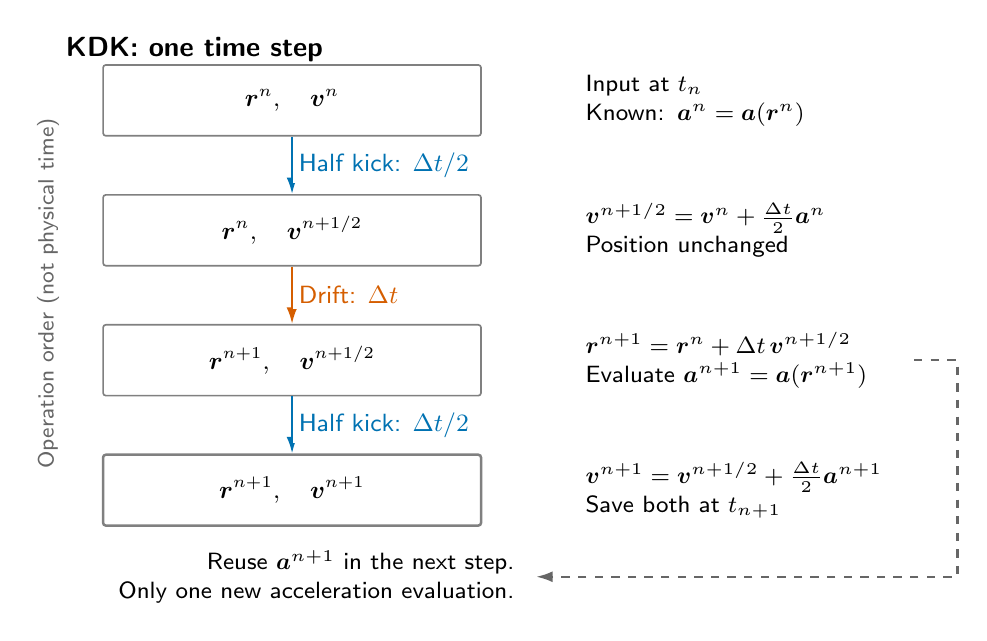
\begin{tikzpicture}[textbook diagram]
  \node[anchor=west,font=\sffamily\bfseries] at (0,0.65) {KDK: one time step};
  \node[state] (in) at (3,0) {$\boldsymbol r^n,\quad\boldsymbol v^n$};
  \node[hint,text width=38mm,anchor=west] at (6.6,0) {Input at $t_n$\\Known: $\boldsymbol a^n=\boldsymbol a(\boldsymbol r^n)$};
  \node[state] (kick) at (3,-1.65) {$\boldsymbol r^n,\quad\boldsymbol v^{n+1/2}$};
  \draw[vector,figblue] (in.south) -- node[right,fill=white,inner sep=2pt] {Half kick: $\Delta t/2$} (kick.north);
  \node[hint,text width=41mm,anchor=west] at (6.6,-1.65) {$\boldsymbol v^{n+1/2}=\boldsymbol v^n+\frac{\Delta t}{2}\boldsymbol a^n$\\Position unchanged};
  \node[state] (drift) at (3,-3.30) {$\boldsymbol r^{n+1},\quad\boldsymbol v^{n+1/2}$};
  \draw[vector,figred] (kick.south) -- node[right,fill=white,inner sep=2pt] {Drift: $\Delta t$} (drift.north);
  \node[hint,text width=41mm,anchor=west] at (6.6,-3.30) {$\boldsymbol r^{n+1}=\boldsymbol r^n+\Delta t\,\boldsymbol v^{n+1/2}$\\Evaluate $\boldsymbol a^{n+1}=\boldsymbol a(\boldsymbol r^{n+1})$};
  \node[state,line width=0.9pt] (out) at (3,-4.95) {$\boldsymbol r^{n+1},\quad\boldsymbol v^{n+1}$};
  \draw[vector,figblue] (drift.south) -- node[right,fill=white,inner sep=2pt] {Half kick: $\Delta t/2$} (out.north);
  \node[hint,text width=41mm,anchor=west] at (6.6,-4.95) {$\boldsymbol v^{n+1}=\boldsymbol v^{n+1/2}+\frac{\Delta t}{2}\boldsymbol a^{n+1}$\\Save both at $t_{n+1}$};
  \draw[vector,figgray,dashed] (10.90,-3.30) -- (11.45,-3.30) -- (11.45,-6.05) -- (6.10,-6.05);
  \node[hint,anchor=east,text width=52mm,align=right] at (5.95,-6.05) {Reuse $\boldsymbol a^{n+1}$ in the next step.\\Only one new acceleration evaluation.};
  \node[rotate=90,small label,text=figgray] at (-0.10,-2.45) {Operation order (not physical time)};
\end{tikzpicture}

\captionof{figure}{KDKの1ステップで受け渡す位置・速度・加速度。縦方向は計算操作の順序であり、物理時間軸ではありません。最後の半kickを終えた位置と速度を整数時刻の状態として保存し、新しい加速度を次のステップへ引き継ぎます。}
\end{minipage}
\clearpage
\noindent{\Large\sffamily\bfseries RK4の4段階}\par\medskip
\noindent{\small 本文の対応箇所：1.6.1節}
\par\bigskip
\noindent\begin{minipage}{\linewidth}\centering
% Each predicted state starts from y^n; the arrows show dependencies, not a time partition.
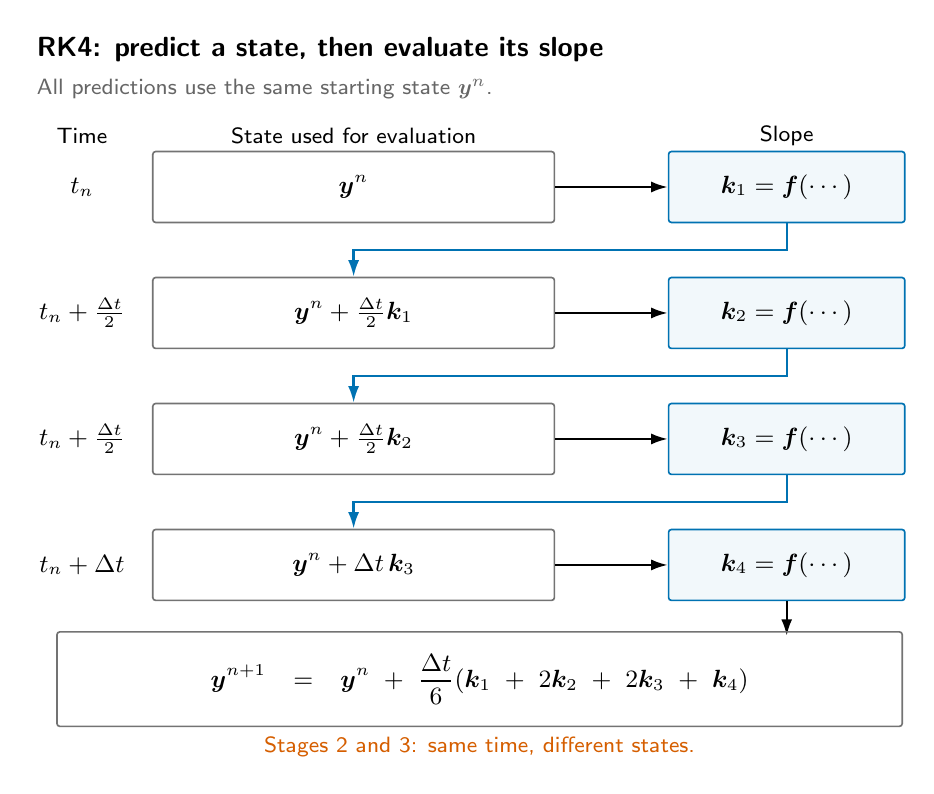
\begin{tikzpicture}[textbook diagram]
  \node[anchor=west,font=\sffamily\bfseries] at (0,0.80) {RK4: predict a state, then evaluate its slope};
  \node[small label,text=figgray,anchor=west] at (0,0.30) {All predictions use the same starting state $\boldsymbol y^n$.};
  \node[small label] at (0.70,-0.30) {Time};
  \node[small label] at (4.15,-0.30) {State used for evaluation};
  \node[small label] at (9.65,-0.30) {Slope};
  \foreach \y/\id in {-0.95/1,-2.55/2,-4.15/3,-5.75/4} {
    \node[draw=black!55,rounded corners=1pt,minimum width=51mm,minimum height=9mm,fill=white] (s\id) at (4.15,\y) {};
    \node[draw=figblue,rounded corners=1pt,minimum width=30mm,minimum height=9mm,fill=figblue!5] (k\id) at (9.65,\y) {$\boldsymbol k_{\id}=\boldsymbol f(\cdots)$};
    \draw[vector] (s\id.east) -- (k\id.west);
  }
  \node at (0.70,-0.95) {$t_n$};
  \node at (0.70,-2.55) {$t_n+\frac{\Delta t}{2}$};
  \node at (0.70,-4.15) {$t_n+\frac{\Delta t}{2}$};
  \node at (0.70,-5.75) {$t_n+\Delta t$};
  \node at (s1) {$\boldsymbol y^n$};
  \node at (s2) {$\boldsymbol y^n+\frac{\Delta t}{2}\boldsymbol k_1$};
  \node at (s3) {$\boldsymbol y^n+\frac{\Delta t}{2}\boldsymbol k_2$};
  \node at (s4) {$\boldsymbol y^n+\Delta t\,\boldsymbol k_3$};
  \foreach \i/\j/\y in {1/2/-1.75,2/3/-3.35,3/4/-4.95} {
    \draw[vector,figblue] (k\i.south) -- (9.65,\y) -- (4.15,\y) -- (s\j.north);
  }
  \node[small label,text=figred] at (5.75,-8.06) {Stages 2 and 3: same time, different states.};
  \draw[vector] (k4.south) -- (9.65,-6.65);
  \node[draw=black!55,rounded corners=1pt,minimum height=12mm,text width=105mm,align=center] at (5.75,-7.20) {$\displaystyle\boldsymbol y^{n+1}=\boldsymbol y^n+\frac{\Delta t}{6}(\boldsymbol k_1+2\boldsymbol k_2+2\boldsymbol k_3+\boldsymbol k_4)$};
\end{tikzpicture}

\captionof{figure}{RK4の予測状態と傾きの依存関係。各予測は同じ基準状態$\yvec^n$から作ります。$\kvec_2$と$\kvec_3$は評価時刻が同じでも、使う予測状態は異なります。矢印は計算の依存関係で、時間を4等分する図ではありません。}
\end{minipage}
\clearpage
\noindent{\Large\sffamily\bfseries 重心と相対位置}\par\medskip
\noindent{\small 本文の対応箇所：2.3.3節}
\par\bigskip
\noindent\begin{minipage}{\linewidth}\centering
% Example M1 = 2 M2. Symbol sizes are labels, not physical body radii.
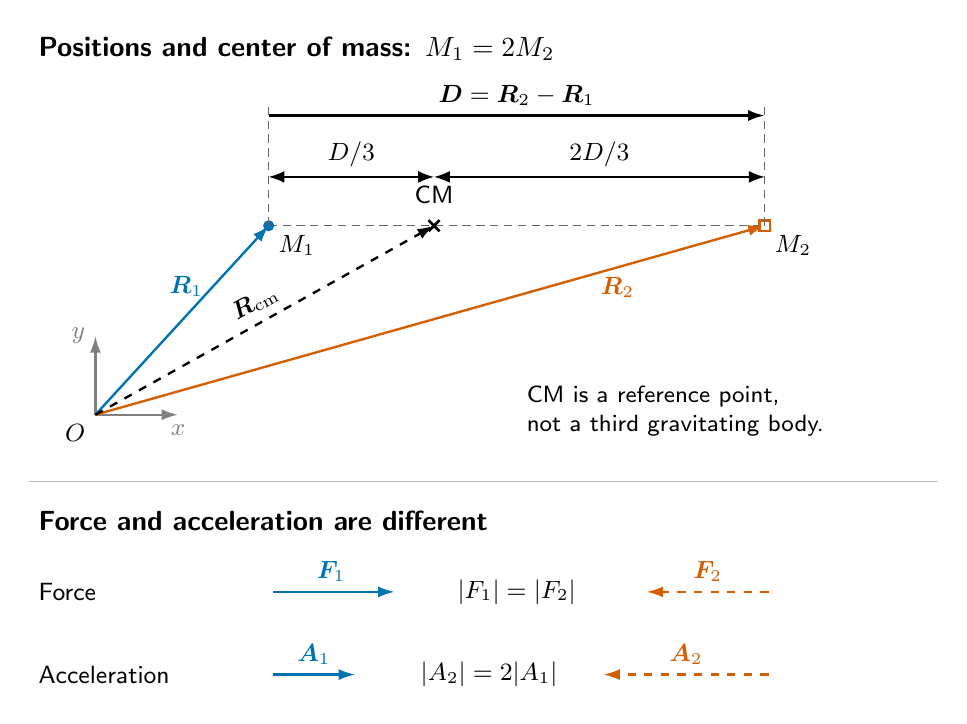
\begin{tikzpicture}[textbook diagram]
  \node[anchor=west,font=\sffamily\bfseries] at (0,4.75) {Positions and center of mass: $M_1=2M_2$};
  \coordinate (O) at (0.85,0.10);
  \coordinate (P) at (3.05,2.5);
  \coordinate (Q) at (9.35,2.5);
  \coordinate (C) at (5.15,2.5);
  \draw[vector,black!50] (O) -- +(1.05,0) node[below] {$x$};
  \draw[vector,black!50] (O) -- +(0,1.0) node[left] {$y$};
  \node[below left] at (O) {$O$};
  \draw[vector,figblue] (O) -- node[left,pos=0.68] {$\boldsymbol R_1$} (P);
  \draw[vector,figred] (O) -- node[below,pos=0.78] {$\boldsymbol R_2$} (Q);
  \draw[vector,black,dashed] (O) -- node[above,pos=0.50,sloped] {$\boldsymbol R_{\rm cm}$} (C);
  \draw[guide] (P) -- (Q);
  \fill[figblue] (P) circle (2.0pt);
  \draw[figred,line width=0.9pt,fill=white] ($(Q)+(-0.065,-0.065)$) rectangle ($(Q)+(0.065,0.065)$);
  \draw[black,line width=1pt] ($(C)+(-0.07,-0.07)$) -- ($(C)+(0.07,0.07)$);
  \draw[black,line width=1pt] ($(C)+(-0.07,0.07)$) -- ($(C)+(0.07,-0.07)$);
  \node[below right] at (P) {$M_1$};
  \node[below right] at (Q) {$M_2$};
  \node[above,yshift=1.5mm] at (C) {CM};
  \draw[vector] (3.05,3.90) -- node[above] {$\boldsymbol D=\boldsymbol R_2-\boldsymbol R_1$} (9.35,3.90);
  \draw[guide] (P) -- (3.05,4.02);
  \draw[guide] (Q) -- (9.35,4.02);
  \draw[<->] (3.05,3.12) -- node[above] {$D/3$} (5.15,3.12);
  \draw[<->] (5.15,3.12) -- node[above] {$2D/3$} (9.35,3.12);
  \node[hint,anchor=west] at (6.2,0.15) {CM is a reference point,\\not a third gravitating body.};
  \draw[black!25] (0,-0.75) -- (11.55,-0.75);
  \node[anchor=west,font=\sffamily\bfseries] at (0,-1.25) {Force and acceleration are different};
  \node[anchor=west] at (0,-2.15) {Force};
  \draw[vector,figblue] (3.1,-2.15) -- (4.65,-2.15) node[above,pos=0.48] {$\boldsymbol F_1$};
  \draw[vector,figred,dashed] (9.4,-2.15) -- (7.85,-2.15) node[above,pos=0.5] {$\boldsymbol F_2$};
  \node at (6.2,-2.15) {$|F_1|=|F_2|$};
  \node[anchor=west] at (0,-3.20) {Acceleration};
  \draw[vector,figblue] (3.1,-3.20) -- (4.15,-3.20) node[above,pos=0.5] {$\boldsymbol A_1$};
  \draw[vector,figred,dashed] (9.4,-3.20) -- (7.30,-3.20) node[above,pos=0.5] {$\boldsymbol A_2$};
  \node at (5.85,-3.20) {$|A_2|=2|A_1|$};
\end{tikzpicture}

\captionof{figure}{質量比$M_1:M_2=2:1$の位置関係。任意の原点$O$と重心CMを区別しています。重心からの距離の比は$1:2$です。下段は力と加速度の違いで、力の大きさは等しくても加速度の大きさは異なります。段をまたいで矢印の長さを比較しません。}
\end{minipage}
\clearpage
\noindent{\Large\sffamily\bfseries 球殻の体積と内側の質量}\par\medskip
\noindent{\small 本文の対応箇所：3.2.1節}
\par\bigskip
\noindent\begin{minipage}{\linewidth}\centering
% A cross-section of a three-dimensional shell, not a material outer boundary.
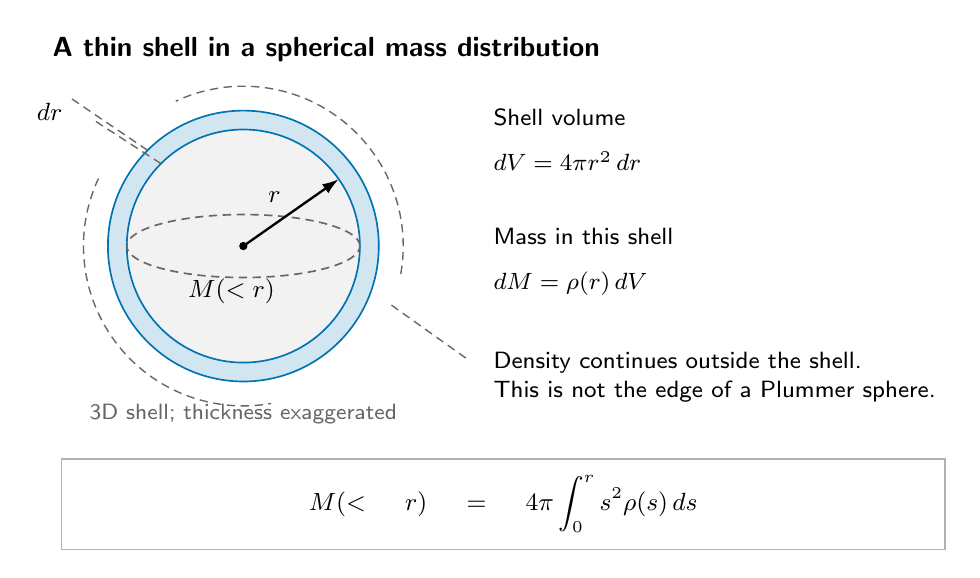
\begin{tikzpicture}[textbook diagram]
  \node[anchor=west,font=\sffamily\bfseries] at (0,4.85) {A thin shell in a spherical mass distribution};
  \coordinate (O) at (2.55,2.35);
  \path[fill=black!5] (O) circle (1.48);
  \path[fill=figblue!18,even odd rule] (O) circle (1.72) (O) circle (1.48);
  \draw[figblue] (O) circle (1.48);
  \draw[figblue] (O) circle (1.72);
  \draw[guide] ($(O)+(-10:2.03)$) arc[start angle=-10,end angle=115,radius=2.03];
  \draw[guide] ($(O)+(155:2.03)$) arc[start angle=155,end angle=280,radius=2.03];
  \draw[figgray,densely dashed] (O) ellipse (1.48 and 0.40);
  \fill (O) circle (1.5pt);
  \draw[vector] (O) -- ($(O)+(35:1.48)$) node[midway,above left] {$r$};
  \draw[guide] ($(O)+(135:1.48)$) -- (0.65,3.95);
  \draw[guide] ($(O)+(135:1.72)$) -- (0.37,4.22);
  \node[anchor=east] at (0.38,4.05) {$dr$};
  \node at (2.4,1.78) {$M(<r)$};
  \node[small label,text=figgray] at (2.55,0.22) {3D shell; thickness exaggerated};
  \node[hint,anchor=west,text width=57mm] at (5.6,3.70) {Shell volume\\[2mm]$dV=4\pi r^2\,dr$};
  \node[hint,anchor=west,text width=57mm] at (5.6,2.15) {Mass in this shell\\[2mm]$dM=\rho(r)\,dV$};
  \node[hint,anchor=west,text width=57mm] at (5.6,0.68) {Density continues outside the shell.\\This is not the edge of a Plummer sphere.};
  \draw[guide] (4.43,1.60) -- (5.4,0.91);
  \node[draw=black!30,fill=white,text width=108mm,align=center,inner sep=6pt] at (5.85,-0.93) {$\displaystyle M(<r)=4\pi\int_0^r s^2\rho(s)\,ds$};
\end{tikzpicture}

\captionof{figure}{3次元の球殻を断面で示した図。色の付いた殻の厚さ$dr$を強調しており、殻の体積は$4\pi r^2dr$です。内側の薄灰色の領域が$M(<r)$に対応します。殻の外にも密度は続き、この円をPlummer球の外縁とはみなしません。}
\end{minipage}
\clearpage
\noindent{\Large\sffamily\bfseries 台形則の高さと幅（既存図の改良）}\par\medskip
\noindent{\small 本文の対応箇所：3.4.2節}
\par\bigskip
\noindent\begin{minipage}{\linewidth}\centering
% Annotation only: the original Matplotlib PDF remains unchanged.
\begin{tikzpicture}[textbook diagram]
  \node[inner sep=0,anchor=south west] (plot) at (0,0) {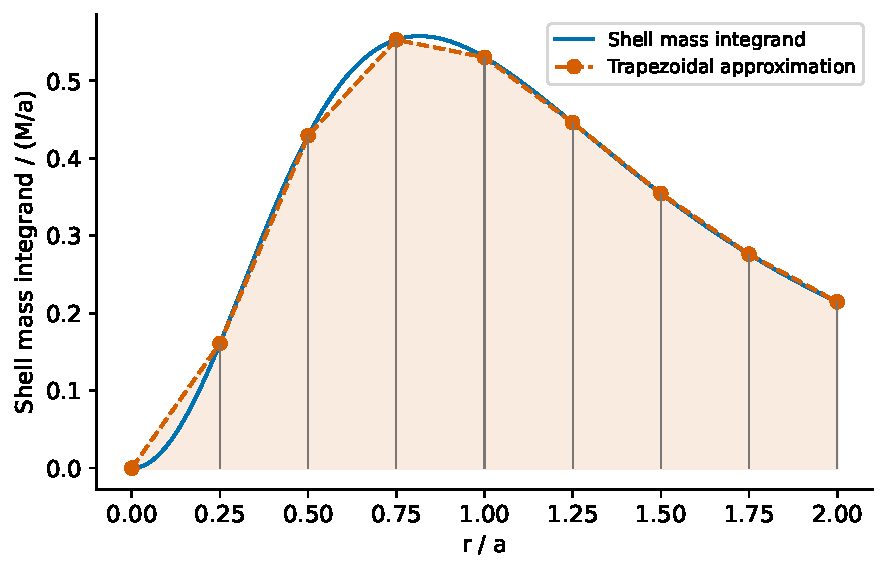
\includegraphics[width=118mm]{figures/ch03_trapezoid.pdf}};
  \begin{scope}[x={(plot.south east)},y={(plot.north west)}]
    \draw[figblue,line width=.85pt] (.645294,.181406) -- (.645294,.784836);
    \draw[figblue,line width=.85pt] (.744648,.181406) -- (.744648,.661074);
    \node[fill=white,inner sep=1.5pt,anchor=east,small label] (gl) at (.618,.64) {$g_j/(M/a)$};
    \draw[guide] (gl.east) -- (.645294,.770);
    \node[fill=white,inner sep=1.5pt,anchor=west,small label] (gr) at (.778,.48) {$g_{j+1}/(M/a)$};
    \draw[guide] (gr.west) -- (.744648,.645);
    \draw[{Latex[length=1.6mm]}-{Latex[length=1.6mm]},figblue] (.645294,.28) -- (.744648,.28);
    \node[small label,fill=white,inner sep=1pt,above] at (.694971,.29) {$\Delta r_j/a$};
  \end{scope}
\end{tikzpicture}

\captionof{figure}{既存の被積分関数と台形近似は変更せず、一つの区間の高さ$g_j,g_{j+1}$と幅$\Delta r_j$を注記しました。軸に合わせて、図中の高さを$M/a$、幅を$a$で規格化しています。}
\end{minipage}
\clearpage
\noindent{\Large\sffamily\bfseries 二分法で残す区間}\par\medskip
\noindent{\small 本文の対応箇所：3.6.3節}
\par\bigskip
\noindent\begin{minipage}{\linewidth}\centering
% Standard [0,5a] bracket: signs correspond to the chapter's half-mass function.
% r_* denotes the root of the function actually evaluated, not an error-free physical radius.
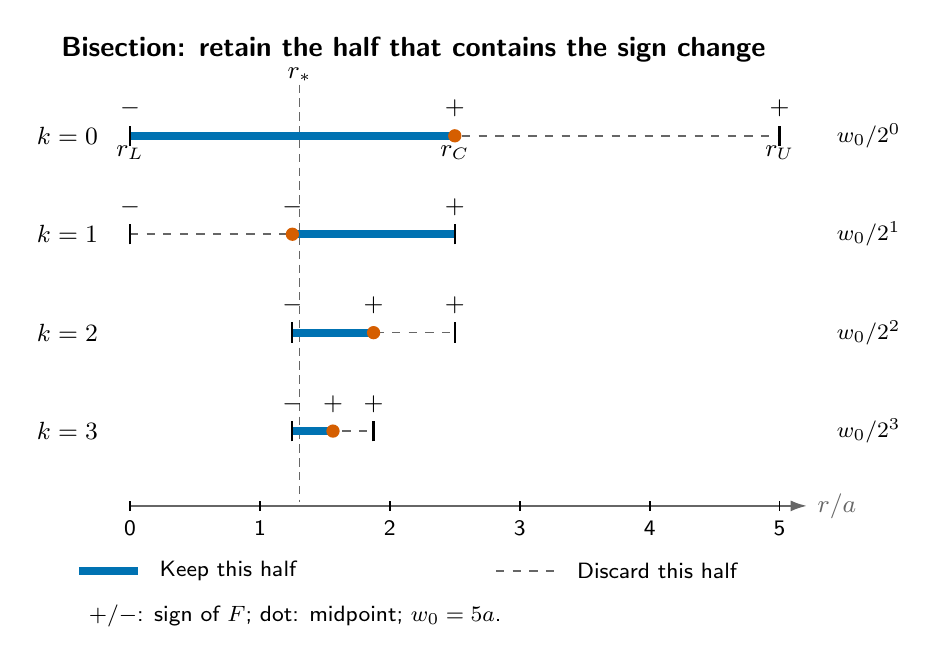
\begin{tikzpicture}[textbook diagram,x=1cm,y=1cm]
  \node[anchor=west,font=\sffamily\bfseries] at (0,1.10) {Bisection: retain the half that contains the sign change};
  \draw[guide] (3.153,0.65) -- (3.153,-4.65);
  \node[above,fill=white,inner sep=1pt] at (3.153,0.65) {$r_*$};
  \foreach \k/\y/\lo/\mid/\hi/\keepL/\keepU/\sign in {
    0/0/0/2.5/5/0/2.5/+,
    1/-1.25/0/1.25/2.5/1.25/2.5/-,
    2/-2.5/1.25/1.875/2.5/1.25/1.875/+,
    3/-3.75/1.25/1.5625/1.875/1.25/1.5625/+} {
    \node[anchor=east] at (.72,\y) {$k=\k$};
    \draw[figgray,dashed] ({1+1.65*\lo},\y) -- ({1+1.65*\hi},\y);
    \draw[figblue,line width=3pt] ({1+1.65*\keepL},\y) -- ({1+1.65*\keepU},\y);
    \foreach \p in {\lo,\hi} {\draw[line width=0.8pt] ({1+1.65*\p},{\y-.13}) -- ({1+1.65*\p},{\y+.13});}
    \fill[figred] ({1+1.65*\mid},\y) circle (2.4pt);
    \node[above,inner sep=3pt] at ({1+1.65*\lo},{\y+.12}) {$-$};
    \node[above,inner sep=3pt] at ({1+1.65*\mid},{\y+.12}) {$\sign$};
    \node[above,inner sep=3pt] at ({1+1.65*\hi},{\y+.12}) {$+$};
    \node[anchor=west,small label] at (9.85,\y) {$w_0/2^{\k}$};
  }
  \node[below] at (1,0) {$r_L$};
  \node[below] at (5.125,0) {$r_C$};
  \node[below] at (9.25,0) {$r_U$};
  \draw[vector,figgray] (1,-4.70) -- (9.6,-4.70) node[right] {$r/a$};
  \foreach \x in {0,1,2,3,4,5} {\draw ({1+1.65*\x},-4.64) -- ({1+1.65*\x},-4.77);\node[below,small label] at ({1+1.65*\x},-4.77) {\x};}
  \draw[figblue,line width=3pt] (0.35,-5.53) -- (1.1,-5.53);
  \node[anchor=west,small label] at (1.25,-5.53) {Keep this half};
  \draw[figgray,dashed] (5.65,-5.53) -- (6.4,-5.53);
  \node[anchor=west,small label] at (6.55,-5.53) {Discard this half};
  \node[small label,anchor=west] at (0.35,-6.10) {$+/-$: sign of $F$; dot: midpoint; $w_0=5a$.};
\end{tikzpicture}

\captionof{figure}{初期区間$[0,5a]$からの二分法の例。点が中点、$+,-$が評価した$F$の符号、太い線が次に残す半区間です。$k$はそれまでの半減回数です。破線$r_*$は評価している数値関数の根であり、元の密度の真の半質量半径と必ずしも一致しません。}
\end{minipage}
\clearpage
\noindent{\Large\sffamily\bfseries 円環と半径の確率密度}\par\medskip
\noindent{\small 本文の対応箇所：4.2.2節}
\par\bigskip
\noindent\begin{minipage}{\linewidth}\centering
% Geometry and two dimensionless density functions, not a simulated snapshot.
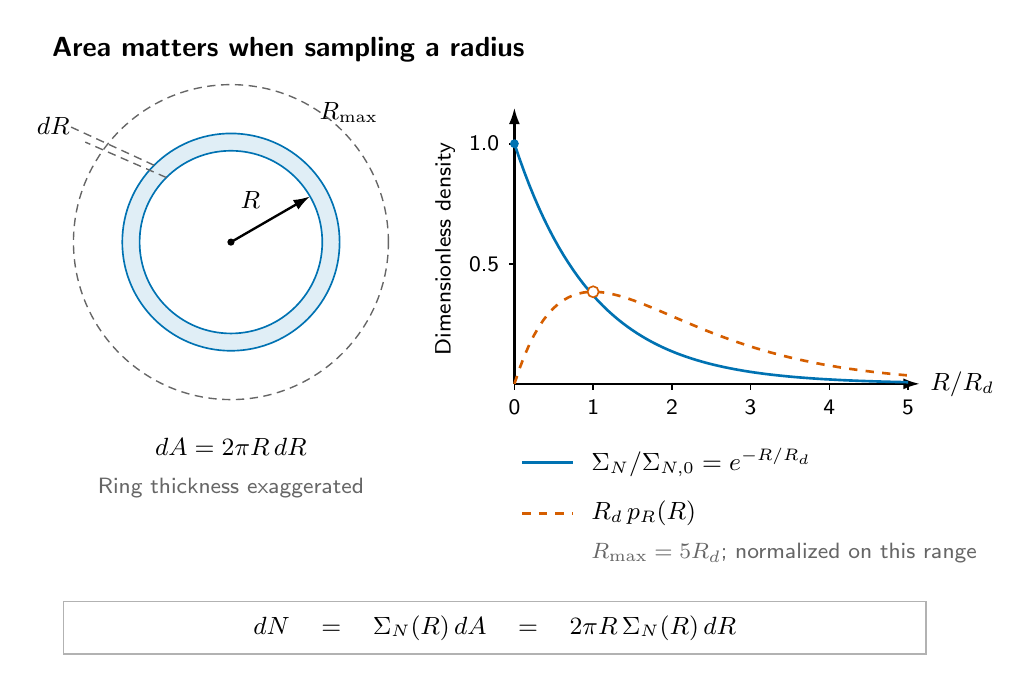
\begin{tikzpicture}[textbook diagram]
  \node[anchor=west,font=\sffamily\bfseries] at (0,4.9) {Area matters when sampling a radius};
  \coordinate (O) at (2.4,2.45);
  \draw[guide] (O) circle (2.0);
  \path[fill=figblue!12,even odd rule] (O) circle (1.38) (O) circle (1.16);
  \draw[figblue] (O) circle (1.16);
  \draw[figblue] (O) circle (1.38);
  \fill (O) circle (1.3pt);
  \draw[vector] (O) -- ($(O)+(30:1.16)$) node[midway,above left] {$R$};
  \draw[guide] ($(O)+(135:1.16)$) -- (0.55,3.72);
  \draw[guide] ($(O)+(135:1.38)$) -- (0.35,3.92);
  \node[anchor=east] at (0.48,3.93) {$dR$};
  \node[anchor=west] at (3.4,4.10) {$R_{\max}$};
  \node at (2.4,-0.15) {$dA=2\pi R\,dR$};
  \node[small label,text=figgray] at (2.4,-0.67) {Ring thickness exaggerated};
  \begin{scope}[shift={(6.0,0.65)},x=1cm,y=3.05cm]
    \draw[vector] (0,0) -- (5.15,0) node[right] {$R/R_d$};
    \draw[vector] (0,0) -- (0,1.15);
    \node[rotate=90,small label] at (-0.88,0.56) {Dimensionless density};
    \foreach \x in {0,1,2,3,4,5} {\draw (\x,0) -- (\x,-0.027); \node[below,small label] at (\x,-0.027) {\x};}
    \foreach \yy in {0.5,1.0} {\draw (0,\yy) -- (-0.065,\yy); \node[left,small label] at (-0.065,\yy) {\yy};}
    \draw[figblue,line width=0.95pt,domain=0:5,samples=81] plot (\x,{exp(-\x)});
    \draw[figred,line width=0.95pt,dashed,domain=0:5,samples=81] plot (\x,{\x*exp(-\x)/(1-6*exp(-5))});
    \fill[figblue] (0,1) circle [radius=1.6pt];
    \draw[figred,fill=white] (1,{exp(-1)/(1-6*exp(-5))}) circle [radius=2pt];
  \end{scope}
  \draw[figblue,line width=0.95pt] (6.10,-0.35) -- (6.75,-0.35);
  \node[anchor=west] at (6.85,-0.35) {$\Sigma_N/\Sigma_{N,0}=e^{-R/R_d}$};
  \draw[figred,line width=0.95pt,dashed] (6.10,-1.00) -- (6.75,-1.00);
  \node[anchor=west] at (6.85,-1.00) {$R_d\,p_R(R)$};
  \node[small label,anchor=west,text=figgray] at (6.85,-1.50) {$R_{\max}=5R_d$; normalized on this range};
  \node[draw=black!30,fill=white,align=center,text width=106mm,inner sep=5pt] at (5.75,-2.45) {$dN=\Sigma_N(R)\,dA=2\pi R\,\Sigma_N(R)\,dR$};
\end{tikzpicture}

\captionof{figure}{円環の面積と半径の確率密度の関係。面密度に$2\pi R$を掛けて半径の分布へ直します。右側は$R_{\max}=5R_d$で規格化した解析的な入力分布で、標本化した粒子の結果ではありません。面密度は中心で最大でも、半径の確率密度は中心で0です。}
\end{minipage}
\clearpage
\noindent{\Large\sffamily\bfseries CDFを逆向きに読む（既存図の改良）}\par\medskip
\noindent{\small 本文の対応箇所：4.5.1節}
\par\bigskip
\noindent\begin{minipage}{\linewidth}\centering
% The original numerical line and analytic CDF are embedded unchanged.
\begin{tikzpicture}[textbook diagram]
  \node[inner sep=0,anchor=south west] (plot) at (0,0) {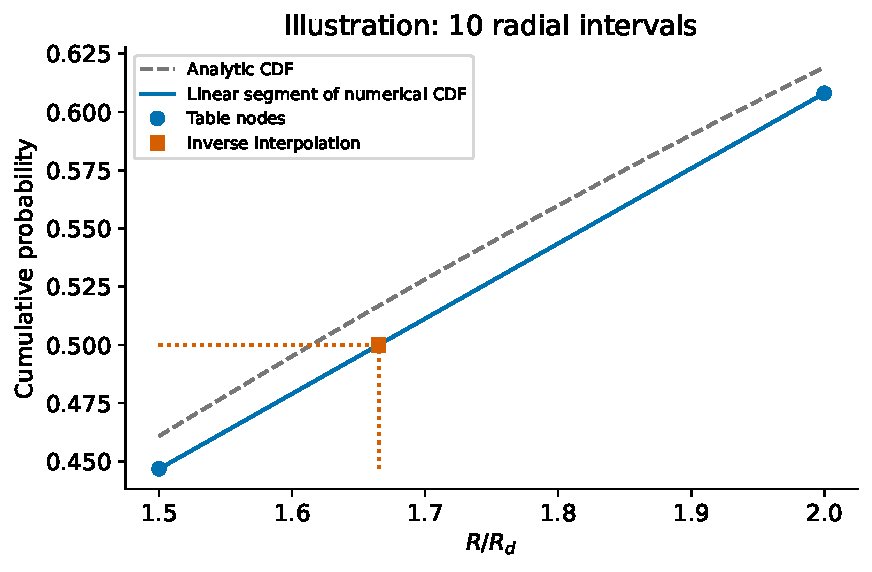
\includegraphics[width=118mm]{figures/ch04_interpolation.pdf}};
  \begin{scope}[x={(plot.south east)},y={(plot.north west)}]
    \draw[vector,figred] (.147,.396700) -- (.422,.396700);
    \draw[vector,figred] (.433970,.380) -- (.433970,.146);
    \node[small label,fill=white,inner sep=1pt,above] at (.245,.402) {$u=0.5$};
    \node[small label,fill=white,inner sep=1pt,anchor=west] at (.453,.196) {$\widehat R(u)/R_d$};
    \node[small label,fill=white,inner sep=1.5pt,anchor=west] (lo) at (.24,.198) {$(R_j,\widehat F_j)$};
    \draw[guide] (lo.west) -- (.182204,.180028);
    \node[small label,fill=white,inner sep=1.5pt,anchor=east] (hi) at (.905,.545) {$(R_{j+1},\widehat F_{j+1})$};
    \draw[guide] (hi.east) -- (.944684,.836223);
  \end{scope}
\end{tikzpicture}

\captionof{figure}{既存の数値CDFの線分と解析CDFを残し、$u$から線分へ、そこから$\widehat R(u)$へたどる矢印を加えました。$(R_j,\widehat F_j)$は表の組であり、横軸では半径を$R_d$で規格化しています。}
\end{minipage}
\clearpage
\noindent{\Large\sffamily\bfseries 中心と星の力の関係}\par\medskip
\noindent{\small 本文の対応箇所：5.2.2節}
\par\bigskip
\noindent\begin{minipage}{\linewidth}\centering
% Dependency arrows, not spatial force vectors.
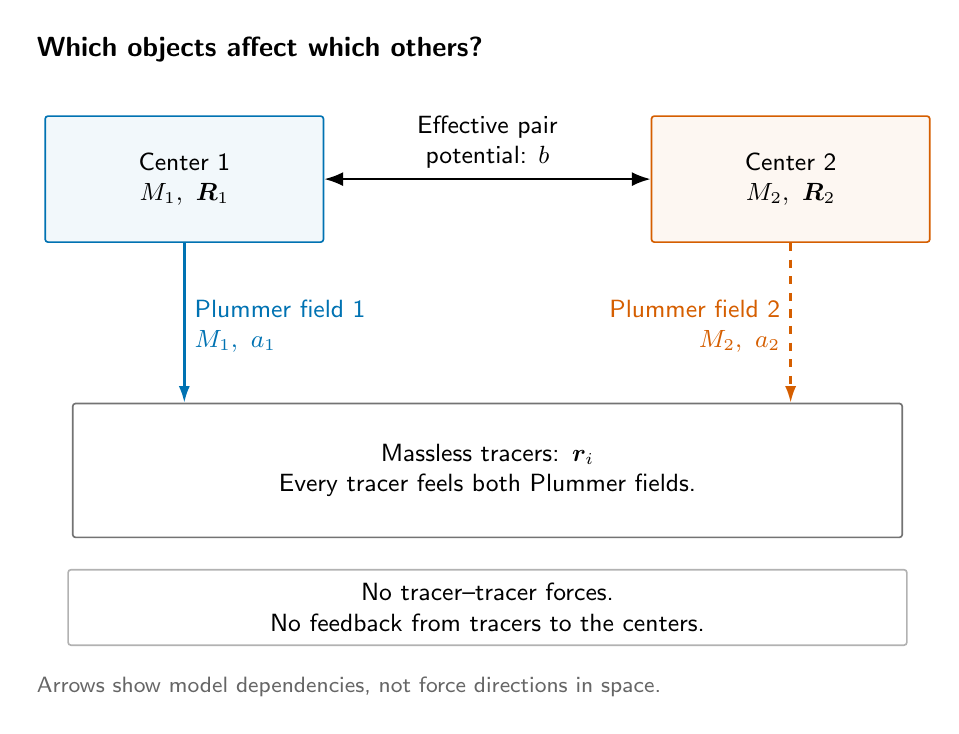
\begin{tikzpicture}[textbook diagram]
  \node[anchor=west,font=\sffamily\bfseries] at (0,4.45) {Which objects affect which others?};
  \node[draw=figblue,fill=figblue!5,rounded corners=1pt,text width=33mm,minimum height=16mm,align=center] (c1) at (2.0,2.80) {Center 1\\$M_1,\ \boldsymbol R_1$};
  \node[draw=figred,fill=figred!5,rounded corners=1pt,text width=33mm,minimum height=16mm,align=center] (c2) at (9.7,2.80) {Center 2\\$M_2,\ \boldsymbol R_2$};
  \draw[{Latex}-{Latex},line width=0.85pt] (c1.east) -- node[above,align=center] {Effective pair\\potential: $b$} (c2.west);
  \node[draw=black!55,fill=white,rounded corners=1pt,text width=103mm,minimum height=17mm,align=center] (stars) at (5.85,-0.90) {Massless tracers: $\boldsymbol r_i$\\Every tracer feels both Plummer fields.};
  \draw[vector,figblue] (c1.south) -- node[right,align=left,pos=.52] {Plummer field 1\\$M_1,\ a_1$} (2.0,-.04);
  \draw[vector,figred,dashed] (c2.south) -- node[left,align=right,pos=.52] {Plummer field 2\\$M_2,\ a_2$} (9.7,-.04);
  \node[draw=black!30,rounded corners=1pt,text width=103mm,align=center,inner sep=5pt] at (5.85,-2.64) {No tracer--tracer forces.\\No feedback from tracers to the centers.};
  \node[small label,text=figgray,anchor=west] at (0,-3.65) {Arrows show model dependencies, not force directions in space.};
\end{tikzpicture}

\captionof{figure}{中心とテスト粒子の間で計算する作用の関係。横の双方向矢印は共通の有効長さ$b$を使う中心間相互作用、下向き矢印は各Plummer場から星への作用です。星から中心への反作用と星同士の重力は計算しません。矢印はモデルの依存関係であり、空間内の力の向きではありません。}
\end{minipage}
\clearpage
\noindent{\Large\sffamily\bfseries 位置と速度の並進}\par\medskip
\noindent{\small 本文の対応箇所：5.4.1節}
\par\bigskip
\noindent\begin{minipage}{\linewidth}\centering
% Separate diagrams for position addition and velocity addition; lengths have different units.
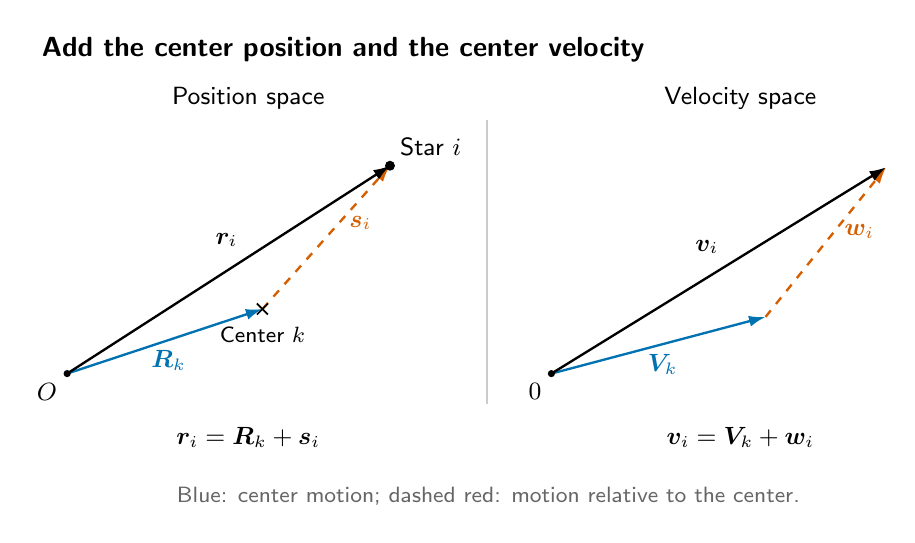
\begin{tikzpicture}[textbook diagram]
  \node[anchor=west,font=\sffamily\bfseries] at (0,4.80) {Add the center position and the center velocity};
  \node at (2.75,4.18) {Position space};
  \node at (9.00,4.18) {Velocity space};
  \coordinate (O) at (0.45,0.68); \coordinate (C) at (2.93,1.50); \coordinate (P) at (4.55,3.32);
  \coordinate (Z) at (6.60,0.68); \coordinate (V) at (9.32,1.40); \coordinate (W) at (10.85,3.30);
  \draw[vector,figblue] (O) -- node[below,pos=.52] {$\boldsymbol R_k$} (C);
  \draw[vector,figred,dashed] (C) -- node[right,pos=.60] {$\boldsymbol s_i$} (P);
  \draw[vector] (O) -- node[above left,pos=.56] {$\boldsymbol r_i$} (P);
  \draw[vector,figblue] (Z) -- node[below,pos=.52] {$\boldsymbol V_k$} (V);
  \draw[vector,figred,dashed] (V) -- node[right,pos=.57] {$\boldsymbol w_i$} (W);
  \draw[vector] (Z) -- node[above left,pos=.53] {$\boldsymbol v_i$} (W);
  \fill (O) circle(1.3pt);\node[below left] at (O) {$O$};
  \fill (Z) circle(1.3pt);\node[below left] at (Z) {$0$};
  \draw[black] ($(C)+(-.07,-.07)$) -- ($(C)+(.07,.07)$);\draw[black] ($(C)+(-.07,.07)$) -- ($(C)+(.07,-.07)$);
  \fill (P) circle(1.8pt);\node[above right] at (P) {Star $i$};
  \node[small label,below,yshift=-1.0mm] at (C) {Center $k$};
  \draw[black!20] (5.78,0.3) -- (5.78,3.9);
  \node at (2.75,-0.13) {$\boldsymbol r_i=\boldsymbol R_k+\boldsymbol s_i$};
  \node at (9.00,-0.13) {$\boldsymbol v_i=\boldsymbol V_k+\boldsymbol w_i$};
  \node[small label,text=figgray] at (5.80,-0.88) {Blue: center motion; dashed red: motion relative to the center.};
\end{tikzpicture}

\captionof{figure}{局所円盤を慣性系へ移す二つのベクトル加算。位置には中心位置$\Rvec_k$、速度には中心速度$\Vvec_k$を加えます。朱色破線は中心に対する局所量です。左右は位置空間と速度空間の図なので、矢印の長さを相互に比較しません。}
\end{minipage}
\clearpage
\noindent{\Large\sffamily\bfseries progradeとretrograde}\par\medskip
\noindent{\small 本文の対応箇所：5.4.2節}
\par\bigskip
\noindent\begin{minipage}{\linewidth}\centering
% Sense-of-rotation sketch. The large curved arrows do NOT depict the center trajectories.
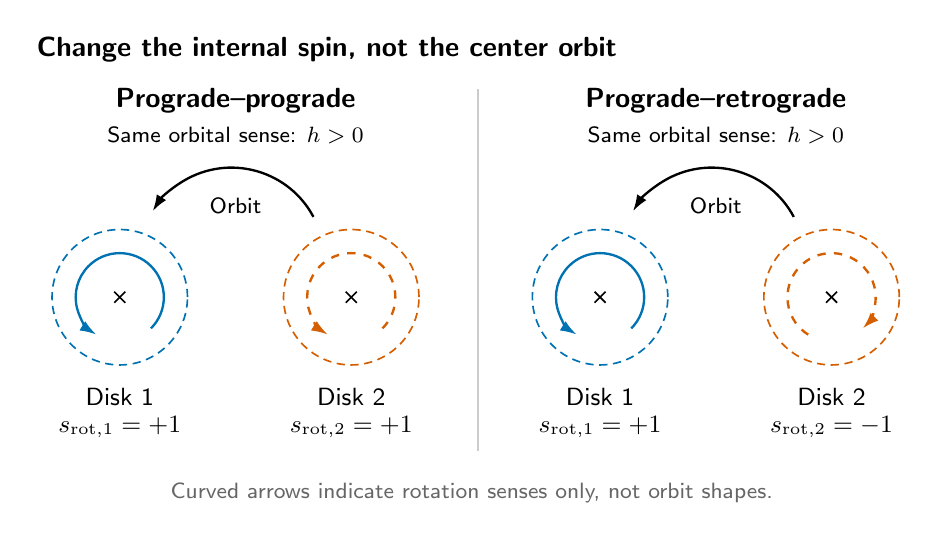
\begin{tikzpicture}[textbook diagram]
  \node[anchor=west,font=\sffamily\bfseries] at (0,4.70) {Change the internal spin, not the center orbit};
  \foreach \shift/\title/\mode in {0/Prograde--prograde/1,6.1/Prograde--retrograde/-1} {
    \begin{scope}[shift={(\shift,0)}]
      \node[font=\sffamily\bfseries] at (2.65,4.05) {\title};
      \node[small label] at (2.65,3.60) {Same orbital sense: $h>0$};
      \draw[vector,black] (3.64,2.57) arc[start angle=28,end angle=148,radius=1.18];
      \node[small label,fill=white,inner sep=1pt] at (2.65,2.71) {Orbit};
      \foreach \cx/\col/\id in {1.18/figblue/1,4.12/figred/2} {
        \draw[\col,densely dashed] (\cx,1.55) circle(.86);
        \draw[black] ({\cx-.07},1.48) -- ({\cx+.07},1.62);\draw[black] ({\cx-.07},1.62) -- ({\cx+.07},1.48);
        \node[below] at (\cx,.52) {Disk \id};
      }
      \draw[vector,figblue] (1.18,1.55) ++(-45:.56) arc[start angle=-45,end angle=238,radius=.56];
      \ifnum\mode=1
        \draw[vector,figred,dashed] (4.12,1.55) ++(-45:.56) arc[start angle=-45,end angle=238,radius=.56];
        \node at (4.12,-.10) {$s_{{\rm rot},2}=+1$};
      \else
        \draw[vector,figred,dashed] (4.12,1.55) ++(238:.56) arc[start angle=238,end angle=-45,radius=.56];
        \node at (4.12,-.10) {$s_{{\rm rot},2}=-1$};
      \fi
      \node at (1.18,-.10) {$s_{{\rm rot},1}=+1$};
    \end{scope}
  }
  \draw[black!20] (5.73,-.40) -- (5.73,4.2);
  \node[small label,text=figgray] at (5.65,-.93) {Curved arrows indicate rotation senses only, not orbit shapes.};
\end{tikzpicture}

\captionof{figure}{軌道の向きを$h>0$に固定した回転方向の比較。左は両円盤がprograde、右は円盤2の内部回転だけがretrogradeです。大きな曲線矢印は軌道の回転の向きを示す記号で、中心軌道の形ではありません。回転は銀河中心に対する局所的な向きで判断します。}
\end{minipage}
\clearpage
\noindent{\Large\sffamily\bfseries 重力と潮汐加速度の差}\par\medskip
\noindent{\small 本文の対応箇所：5.8.2節}
\par\bigskip
\noindent\begin{minipage}{\linewidth}\centering
% Illustration along the line joining two well-separated galaxies.
% Only the companion's gravitational contribution is drawn.
% Arrow lengths use the point-mass far-field form. This is not the close-passage run.
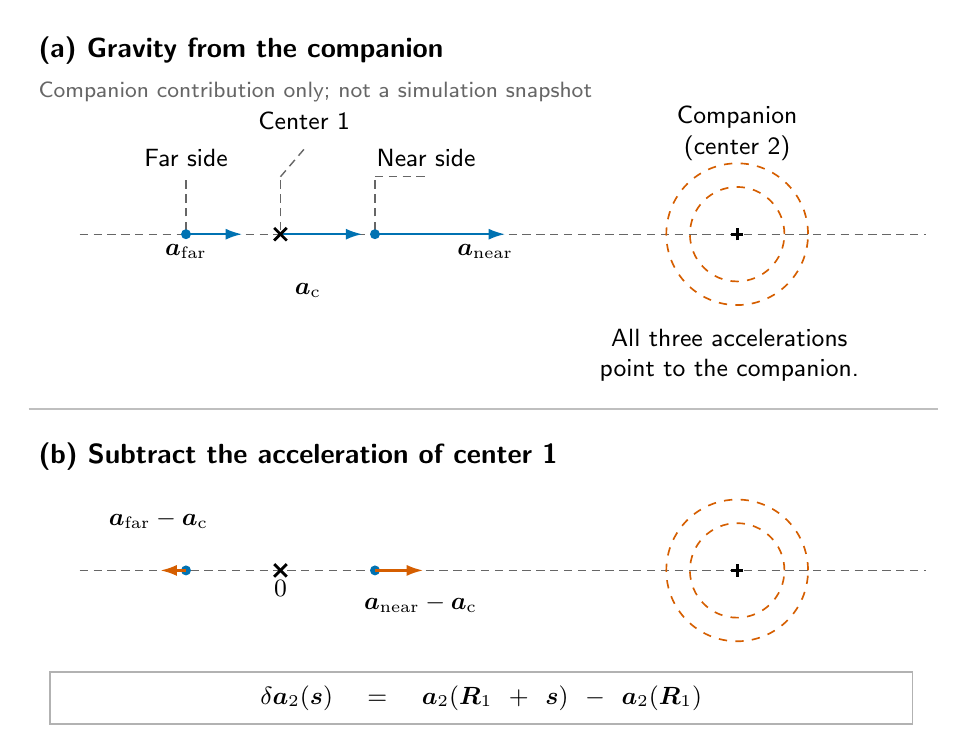
\begin{tikzpicture}[textbook diagram]
  \node[anchor=west,font=\sffamily\bfseries] at (0,4.05) {(a) Gravity from the companion};
  \node[small label,anchor=west,text=figgray] at (0,3.52) {Companion contribution only; not a simulation snapshot};
  \draw[guide] (0.65,1.72) -- (11.40,1.72);
  \foreach \x/\len/\lab in {2/0.71429/far,3.2/1.04043/c,4.4/1.65406/near} {
    \draw[vector,figblue] (\x,1.72) -- ++(\len,0);
    \draw[guide] (\x,1.77) -- (\x,2.45);
  }
  \fill[figblue] (2,1.72) circle (1.8pt);
  \fill[figblue] (4.4,1.72) circle (1.8pt);
  \draw[black,line width=1pt] (3.12,1.64) -- (3.28,1.80);
  \draw[black,line width=1pt] (3.12,1.80) -- (3.28,1.64);
  \node[above] at (2.0,2.45) {Far side};
  \node[above] at (3.5,2.92) {Center 1};
  \draw[guide] (3.2,2.45) -- (3.5,2.80);
  \node[above] at (5.05,2.45) {Near side};
  \draw[guide] (4.4,2.45) -- (5.05,2.45);
  \node[below] at (2.0,1.72) {$\boldsymbol a_{\rm far}$};
  \node[below,yshift=-5mm] at (3.55,1.72) {$\boldsymbol a_{\rm c}$};
  \node[below] at (5.80,1.72) {$\boldsymbol a_{\rm near}$};
  \draw[figred,dashed] (9.0,1.72) circle (0.60);
  \draw[figred,dashed] (9.0,1.72) circle (0.90);
  \draw[black,line width=1pt] (8.92,1.72) -- (9.08,1.72);
  \draw[black,line width=1pt] (9,1.64) -- (9,1.80);
  \node[align=center] at (9,3.0) {Companion\\(center 2)};
  \node[align=center] at (8.9,0.18) {All three accelerations\\point to the companion.};
  \draw[black!25] (0,-0.50) -- (11.55,-0.50);
  \node[anchor=west,font=\sffamily\bfseries] at (0,-1.10) {(b) Subtract the acceleration of center 1};
  \draw[guide] (0.65,-2.55) -- (11.40,-2.55);
  \fill[figblue] (2,-2.55) circle (1.8pt);
  \fill[figblue] (4.4,-2.55) circle (1.8pt);
  \draw[black,line width=1pt] (3.12,-2.63) -- (3.28,-2.47);
  \draw[black,line width=1pt] (3.12,-2.47) -- (3.28,-2.63);
  \draw[vector,figred] (2,-2.55) -- (1.67386,-2.55);
  \draw[vector,figred] (4.4,-2.55) -- (5.01363,-2.55);
  \node[above] at (1.65,-2.15) {$\boldsymbol a_{\rm far}-\boldsymbol a_{\rm c}$};
  \node[below] at (4.98,-2.73) {$\boldsymbol a_{\rm near}-\boldsymbol a_{\rm c}$};
  \node[below] at (3.2,-2.55) {$0$};
  \draw[figred,dashed] (9,-2.55) circle (0.60);
  \draw[figred,dashed] (9,-2.55) circle (0.90);
  \draw[black,line width=1pt] (8.92,-2.55) -- (9.08,-2.55);
  \draw[black,line width=1pt] (9,-2.63) -- (9,-2.47);
  \node[draw=black!30,fill=white,text width=106mm,align=center,inner sep=5pt] at (5.75,-4.17) {$\delta\boldsymbol a_2(\boldsymbol s)=\boldsymbol a_2(\boldsymbol R_1+\boldsymbol s)-\boldsymbol a_2(\boldsymbol R_1)$};
\end{tikzpicture}

\captionof{figure}{相手銀河が十分遠い配置での説明図。上段は相手からの加速度、下段は銀河1の中心加速度を引いた差です。銀河1自身の重力は描いていません。$a_1=a_2=b$で中心加速度が対応する場合を考えています。近点8 kpcの標準計算のスナップショットではありません。}
\end{minipage}
\clearpage
\noindent{\Large\sffamily\bfseries 近点からの時間をそろえる}\par\medskip
\noindent{\small 本文の対応箇所：6.2.3節}
\par\bigskip
\noindent\begin{minipage}{\linewidth}\centering
% Schematic timing only. The benchmark's pericenter is measured from sampled center positions.
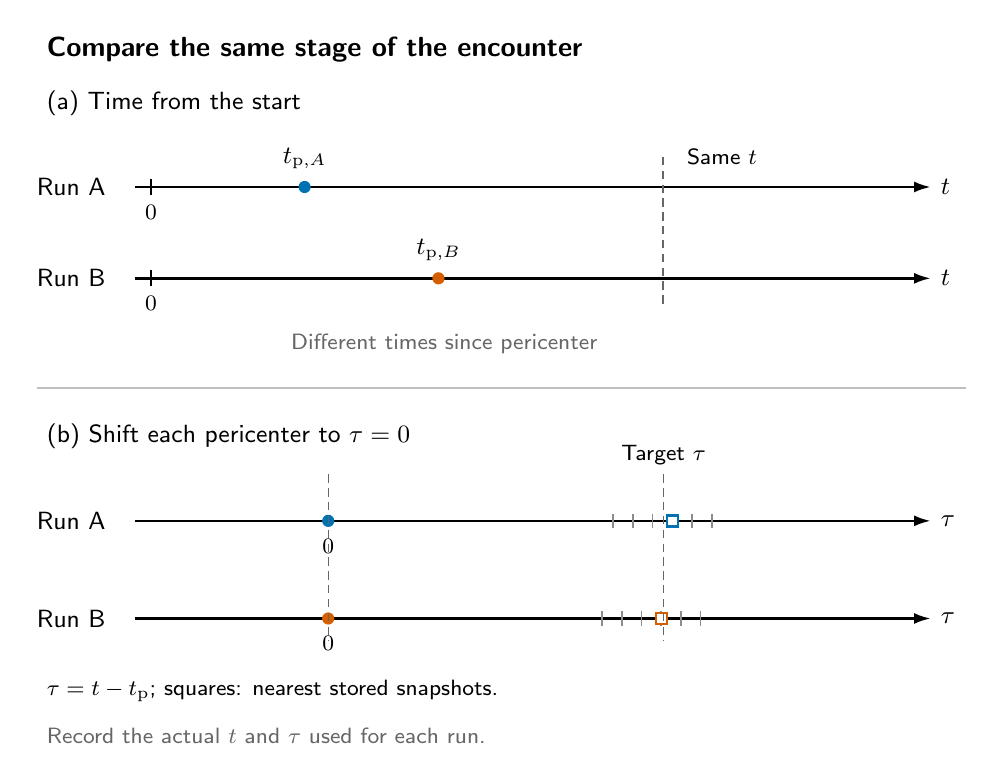
\begin{tikzpicture}[textbook diagram]
  \node[anchor=west,font=\sffamily\bfseries] at (0,4.73) {Compare the same stage of the encounter};
  \node[anchor=west] at (0,4.04) {(a) Time from the start};
  \foreach \y/\tag/\p/\col in {2.98/A/3.4/figblue,1.82/B/5.1/figred} {
    \node[anchor=east] at (1.0,\y) {Run \tag};
    \draw[vector] (1.25,\y) -- (11.35,\y) node[right] {$t$};
    \draw (1.45,{\y-.10}) -- (1.45,{\y+.10});\node[below,small label] at (1.45,{\y-.10}) {$0$};
    \fill[\col] (\p,\y) circle (2.2pt);
    \node[above] at (\p,{\y+.10}) {$t_{{\rm p},\tag}$};
  }
  \draw[guide] (7.95,1.5) -- (7.95,3.43);
  \node[small label,anchor=west] at (8.13,3.36) {Same $t$};
  \node[small label,text=figgray,anchor=west] at (3.10,.99) {Different times since pericenter};
  \draw[black!25] (0,.43) -- (11.80,.43);
  \node[anchor=west] at (0,-.18) {(b) Shift each pericenter to $\tau=0$};
  \foreach \y/\tag/\col/\sel in {-1.26/A/figblue/8.07,-2.50/B/figred/7.93} {
    \node[anchor=east] at (1.0,\y) {Run \tag};
    \draw[vector] (1.25,\y) -- (11.35,\y) node[right] {$\tau$};
    \fill[\col] (3.7,\y) circle (2.2pt);
    \node[below,small label] at (3.7,{\y-.10}) {$0$};
    \foreach \delta in {-.75,-.50,-.25,0,.25,.50} {\draw[black!45] ({\sel+\delta},{\y-.09}) -- ({\sel+\delta},{\y+.09});}
    \draw[\col,fill=white,line width=.9pt] ({\sel-.07},{\y-.07}) rectangle ({\sel+.07},{\y+.07});
  }
  \draw[guide] (3.7,-.67) -- (3.7,-2.78);
  \draw[guide] (7.96,-.67) -- (7.96,-2.78);
  \node[small label,above] at (7.96,-.68) {Target $\tau$};
  \node[small label,anchor=west] at (0,-3.42) {$\tau=t-t_{\rm p}$; squares: nearest stored snapshots.};
  \node[small label,text=figgray,anchor=west] at (0,-3.99) {Record the actual $t$ and $\tau$ used for each run.};
\end{tikzpicture}

\captionof{figure}{開始からの時刻$t$と、近点からの経過時間$\tau=t-t_{\rm p}$の違い。下段では各近点を$\tau=0$へそろえています。小目盛りは保存時刻、四角は目標に最も近い保存時刻です。配置と目盛りは説明用で、実測の時間間隔を表していません。}
\end{minipage}
\clearpage
\noindent{\Large\sffamily\bfseries 背景応答と近似摩擦項}\par\medskip
\noindent{\small 本文の対応箇所：7.2.2節}
\par\bigskip
\noindent\begin{minipage}{\linewidth}\centering
% No wake image is fabricated: the uncomputed response and implemented force are kept separate.
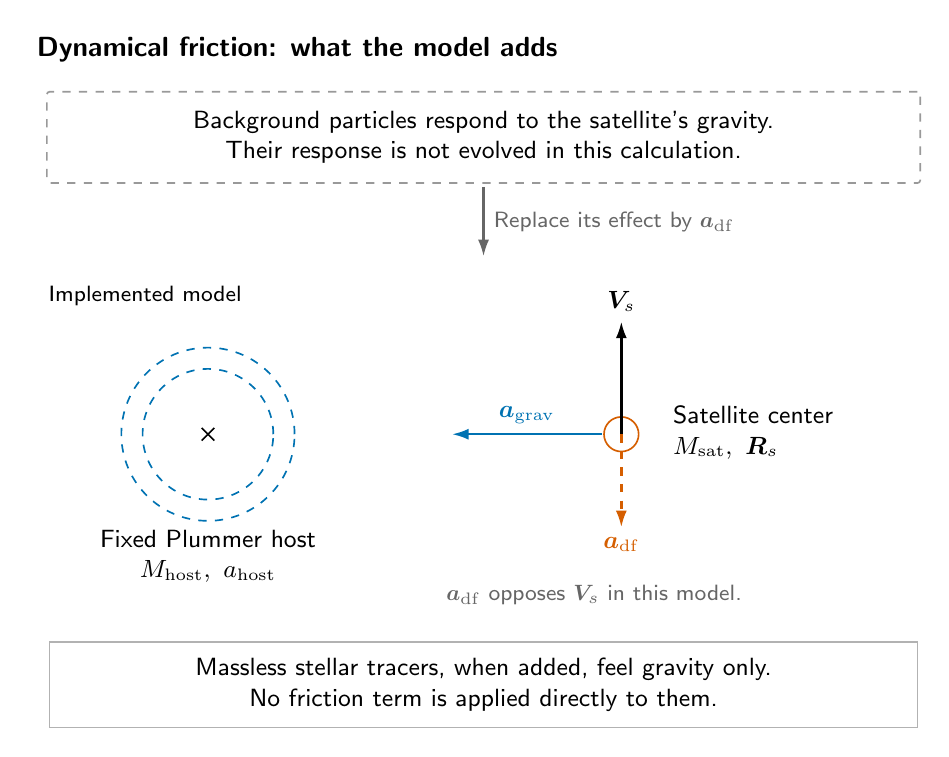
\begin{tikzpicture}[textbook diagram]
  \node[anchor=west,font=\sffamily\bfseries] at (0,4.77) {Dynamical friction: what the model adds};
  \node[draw=black!40,dashed,rounded corners=1pt,text width=106mm,align=center,inner sep=7pt] at (5.8,3.65) {Background particles respond to the satellite's gravity.\\Their response is not evolved in this calculation.};
  \draw[vector,figgray] (5.8,3.02) -- node[right,small label] {Replace its effect by $\boldsymbol a_{\rm df}$} (5.8,2.14);
  \node[small label,anchor=west] at (.15,1.64) {Implemented model};
  \coordinate (H) at (2.3,-.12); \coordinate (S) at (7.55,-.12);
  \draw[figblue,dashed] (H) circle (.83);\draw[figblue,dashed] (H) circle (1.10);
  \draw (2.22,-.20) -- (2.38,-.04);\draw (2.22,-.04) -- (2.38,-.20);
  \node[align=center] at (2.3,-1.67) {Fixed Plummer host\\$M_{\rm host},\ a_{\rm host}$};
  \draw[figred] (S) circle (.22);
  \draw[vector,figblue] ($(S)+(-.25,0)$) -- (5.40,-.12) node[midway,above] {$\boldsymbol a_{\rm grav}$};
  \draw[vector] (S) -- (7.55,1.31) node[above] {$\boldsymbol V_s$};
  \draw[vector,figred,dashed] (S) -- (7.55,-1.30) node[below] {$\boldsymbol a_{\rm df}$};
  \node[align=left,anchor=west] at (8.08,-.10) {Satellite center\\$M_{\rm sat},\ \boldsymbol R_s$};
  \node[small label,text=figgray,anchor=west] at (5.2,-2.16) {$\boldsymbol a_{\rm df}$ opposes $\boldsymbol V_s$ in this model.};
  \node[draw=black!30,text width=106mm,align=center,inner sep=6pt] at (5.8,-3.30) {Massless stellar tracers, when added, feel gravity only.\\No friction term is applied directly to them.};
\end{tikzpicture}

\captionof{figure}{背景応答と実装する摩擦項の区別。上段の背景応答を直接計算する代わりに、下段では衛星中心へ$\avec_{\rm df}$を与えます。静止した平均背景に対して、摩擦は衛星速度と逆向きです。追加する質量ゼロの星には摩擦を直接掛けません。矢印の長さは力の実測値ではありません。}
\end{minipage}
\clearpage
\end{document}
